% !TeX document-id = {3ffda977-020f-403a-a748-6559a1e64ed1}
% !TeX TXS-program:compile = txs:///pdflatex/[--shell-escape]
% % !TEX TS-program = xelatex
% !TEX encoding = UTF-8 Unicode


% Spring 2020 - Summer 2020 - Fall 2020 - SPring 2021
% Tristan Hill, May 07, 2020 - June 12, 2020 - July 08, 2020 - Novemeber 02, 2020 - March 28, 2021
% Module Name: - Data Acquisition
% Topic 3 - Sampling and Aliasing

\documentclass[fleqn]{beamer} % for presentation (has nav buttons at bottom)

%\usepackage{/home/thill/Documents/lectures/measurements_lectures/measurements_lectures}
\usepackage{/home/tntech.edu/thill/courses/measurements/lectures/measurements_lectures}

\author{ME3023 - Measurements in Mechanical Systems} % original formatting from Mike Renfro, September 21, 2004

%\newcommand{\MNUM}{9\hspace{2mm}} % Module number - The module number should be phased out...
\newcommand{\TNUM}{3\hspace{2mm}} % Topic number - Topic numbers are going to stay
\newcommand{\moduletitle}{Data Acquisition}
\newcommand{\topictitle}{Sampling and Aliasing} 

\newcommand{\sectiontitleI}{Sampling}
\newcommand{\sectiontitleII}{The Aliasing Phenomenon}
\newcommand{\sectiontitleIII}{Example by Hand}
\newcommand{\sectiontitleIV}{MATLAB Example}

\newcommand{\btVFill}{\vskip0pt plus 1filll}


% custom box
\newsavebox{\mybox}

\title{Lecture Module - \moduletitle}

\date{Mechanical Engineering\vspc Tennessee Technological University}

\begin{document}

\lstset{language=MATLAB,basicstyle=\ttfamily\small,showstringspaces=false}

\frame{\titlepage \center\begin{framed}\Large \textbf{Topic \TNUM - \topictitle}\end{framed} \vspace{5mm}}

% Section 0: Outline
\frame{
\large \textbf{Topic \TNUM - \topictitle} \vspace{3mm}\\

\begin{itemize}

	\item \sectiontitleI    \vspc % Section I
	\item \sectiontitleII 	\vspc % Section II
	\item \sectiontitleIII 	\vspc %Section III
	\item \sectiontitleIV 	\vspc %Section IV
%	\item \sectiontitleV 	\vspc %Section IV

\end{itemize}

}

% Section I:
\section{\sectiontitleI}

	% Section I - Frame I:
	\begin{frame}[label=sectionI] \small
		\frametitle{\sectiontitleI}
		\vspace{5mm}
		...
		A discrete time signal usually
		results from the sampling of a continuous variable at repeated finite time intervals.
		...	
		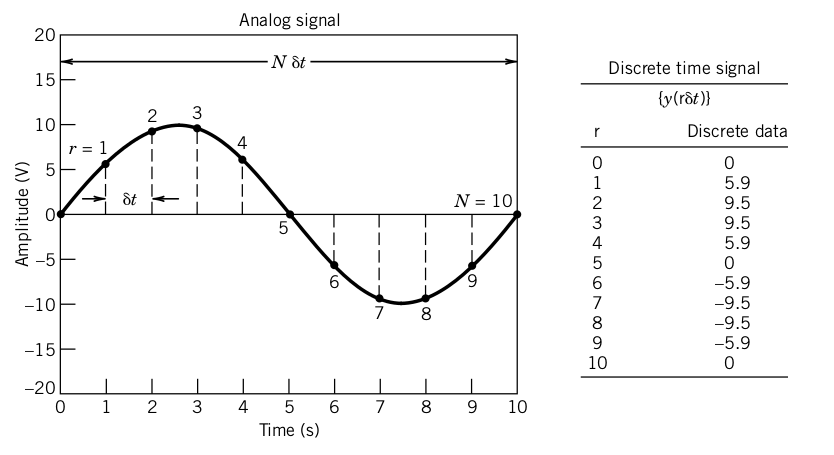
\includegraphics[scale=.3]{sampling_fig7_1.png}
	
		\btVFill
		\tiny{Text,Figure: Theory and Design for Mechanical Measurements Ch. 7}
	\end{frame}
	
	% Section I - Frame II:
	\begin{frame}[label=sectionI] \small
	\frametitle{\sectiontitleI}
	

	\btVFill
	\tiny{some reference}
\end{frame}

\section{\sectiontitleII}	

% Section II - Frame I
\begin{frame}[label=sectionII] \small
\frametitle{\sectiontitleII}
\bigskip
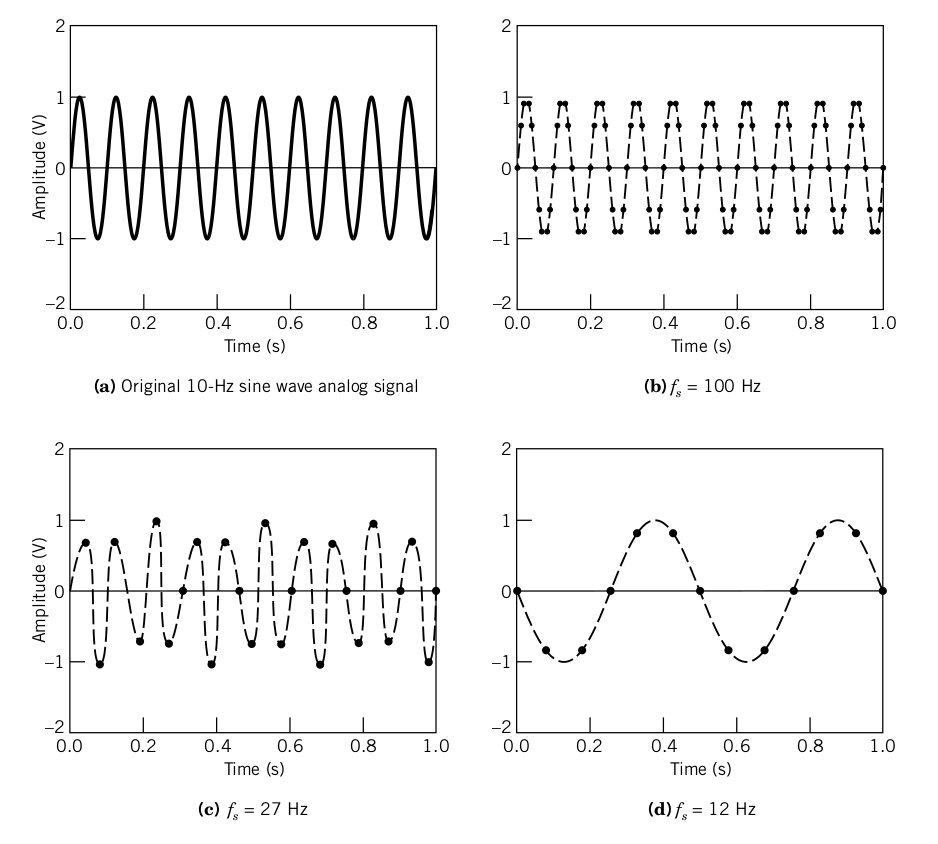
\includegraphics[scale=.2]{aliasing_fig7_2.png}


\btVFill
\tiny{Figure: Theory and Design for Mechanical Measurements Ch. 7}		

\end{frame}
	
\section{\sectiontitleIII}	

% Section III - Frame I
\begin{frame}[label=sectionIII] \small
\frametitle{\sectiontitleIII}
\bigskip

\includegraphics[scale=.35]{cartesian_6x12.png}


\btVFill
\tiny{Image: T.Hill}		

\end{frame}

% Section III - Frame II
\begin{frame}[label=sectionIII] \small
\frametitle{\sectiontitleIII}
\bigskip


\btVFill
\tiny{some reference}	
\end{frame}

\section{\sectiontitleIV}	

% Section IV - Frame I
\begin{frame}[containsverbatim,label=sectionIV] \small
\frametitle{\sectiontitleIV}
\bigskip

\begin{lstlisting}
% ME3023 - Tennessee Technological University 
% Tristan Hill - October 10, 2019 - April 14, 2021
% Data Acquisition Topic 3 - Sampling and Aliasing

clear variables; close all; clc

% simulate a continuous signal
A1=5; f1=3;
w1=2*pi*f1;

dt_sim=0.001; t_stop=6;
t_sim=0:dt_sim:t_stop;
y_sim=A1*sin(w1*t_sim);
\end{lstlisting}


%\tiny{MATLAB cod}	
\end{frame}

% Section IV - Frame II
\begin{frame}[containsverbatim,label=sectionIV] \small
\frametitle{\sectiontitleIV}
\bigskip

\begin{lstlisting}

% simulate sampling the signal
dt_sam = 0.3;
t_sam=0:dt_sam:t_stop;
y_sam=A1*sin(w1*t_sam);

% show the figure
figure(1); hold on
plot(t_sim,y_sim,'-',t_sam,y_sam,'o')
axis([0 t_stop -1.2*A1 1.2*A1])
grid on
\end{lstlisting}


\btVFill
\tiny{MATLAB code: T. Hill}	
\end{frame}

\end{document}
